\documentclass{article}

% Drop in the real neurips_2024.sty before submission and replace the line below.
\usepackage[margin=1in]{geometry}

\usepackage[utf8]{inputenc}
\usepackage[T1]{fontenc}
\usepackage{hyperref}
\usepackage{url}
\usepackage{booktabs}
\usepackage{amsmath}
\usepackage{amsfonts}
\usepackage{amssymb}
\usepackage{graphicx}
\usepackage{lmodern}

\title{Credit Card Fraud Detection with Benford's Law\\and Sequence-Inspired Features}

\author{%
  Dutch Casadaban, Brandon Buckley, Carson Phillips, Devon Li\\
  Auburn University\\
  COMP 5630 / 6630, Spring 2026
}

\begin{document}
\maketitle

\begin{abstract}
We train seven supervised classifiers and one unsupervised anomaly detector on the public ULB credit card fraud dataset and compare their behaviour on a time-ordered 70/10/20 split. The progression runs from an unregularised logistic regression baseline through class-weighted variants, gradient-boosted trees with a held-out hyperparameter sweep, a scaled multi-layer perceptron, and an autoencoder trained only on legitimate transactions. We test two feature-engineering ideas that come from outside the usual machine learning toolkit. The first is leading-digit features derived from Benford's Law. The second is rolling time-window aggregates inspired by Stripe's public description of their Payments Foundation Model. The scaled MLP wins on both headline metrics: test AUPRC of 0.816 and precision of 0.833 at 80\% recall. A tuned LightGBM with Benford features reaches AUPRC 0.808. Benford features give a consistent lift across linear and tree models. The time-window features hurt both, which argues against applying Stripe's sequence-first lesson to a dataset that lacks per-card identifiers. Fraudulent transaction amounts are 6.9$\times$ more distant from Benford's predicted distribution than legitimate amounts in terms of chi-square, a fingerprint that holds up independent of any classifier.
\end{abstract}

\section{Introduction}

Credit card fraud detection is a supervised learning problem that is harder than it looks. The dataset is large, the positive class is small, and the operating point that matters in production is not the one most papers report. A fraud team picks a threshold, commits to the false-positive rate they can tolerate, and lives with whatever precision falls out. AUPRC is a useful scalar summary but it can mislead at that threshold in both directions. Throughout this report we track AUPRC for ranking quality and precision at 80\% recall as a stand-in for deployment quality.

We picked the ULB credit card fraud dataset \cite{dalpozzolo2018} because it is the standard public benchmark, and because its anonymised PCA features force any gains to come from modelling choices rather than from hand-crafted domain knowledge. Three things shaped the project.

First, Stripe's engineering team published a piece describing their Payments Foundation Model, a large transformer trained on sequences of tokenised transactions, which they credit with an overnight jump in card-testing detection rate from 59\% to 97\% on large merchants \cite{stripeflywheel2024}. The architectural details are proprietary but the core claim is simple: fraud is a sequential and bursty phenomenon that per-transaction models undersell. We wanted to see whether a weak, small-scale version of this thesis is testable on a public dataset with no card identifiers.

Second, Benford's Law is a forensic accounting tool with a long history of catching fabricated numerical data \cite{nigrini2012}. It says the leading digit $d$ of many real-world distributions follows $P(d) = \log_{10}(1 + 1/d)$, so digit 1 appears about 30\% of the time and digit 9 only about 4.6\%. Fabricated numbers rarely obey it. We wanted to know whether leading-digit features help a fraud classifier, and whether the Benford gap is visible in the training data itself before any model is involved.

Third, the course rubric asks for a staircase of models with explicit comparisons, and both the Stripe and Benford ideas fit that staircase cleanly.

Our contributions are empirical. Benford features give a small but consistent lift to both linear and tree models. Time-window aggregates, our weak proxy for Stripe's sequential features, hurt on this dataset, which we attribute to the absence of per-card grouping in the ULB data. Hyperparameter tuning on a time-ordered validation slice can actively hurt test performance when the validation and test distributions drift (Section~\ref{sec:discussion}). And we report a simple diagnostic that survives without any classifier at all: the chi-square distance from Benford's predicted distribution is 6.9$\times$ larger for fraudulent amounts than for legitimate amounts.

\subsection{Problem statement and SMART objectives}

We predict a binary label \texttt{Class} $\in \{0, 1\}$ for each transaction, where 1 indicates fraud. The objectives below are written to be specific, measurable, achievable, relevant, and time-bound (SMART):

\begin{itemize}
\item \textbf{Specific.} Binary classification of credit card transactions in the public ULB dataset as fraudulent or legitimate, using a time-ordered 70/10/20 split.
\item \textbf{Measurable.} AUPRC (area under the precision-recall curve), ROC-AUC, precision at 80\% recall, and best-F1 on a held-out test slice. We target AUPRC $\geq 0.80$ and precision at 80\% recall $\geq 0.75$.
\item \textbf{Achievable.} Published baselines on this dataset report AUPRC in the 0.75 to 0.85 range for strong supervised models. Our target sits in the middle of that range.
\item \textbf{Relevant.} Maps directly to the real-world problem of preventing card-not-present fraud at a payments processor. Stripe's recent public results \cite{stripeflywheel2024} make this framing current.
\item \textbf{Time-bound.} Complete end-to-end in a single Google Colab session, reproducible from a GitHub clone with \texttt{Run All}.
\end{itemize}

\section{Related Work}

\paragraph{Sequence-aware fraud models.} Stripe's public post \cite{stripeflywheel2024} is the closest thing to a modern industry reference. They describe a transformer trained on billions of transactions that produces per-transaction embeddings, then run downstream classifiers on sequences of those embeddings to decide whether an entity is under attack in real time. The architectural details (model size, training objective, evaluation splits) are not disclosed. They give no baselines. The gains they report are large but not directly reproducible. We treat their work as motivation rather than a reproducible target.

\paragraph{Classical fraud detection on ULB.} Dal Pozzolo et al.~\cite{dalpozzolo2018} published the original dataset description alongside a realistic cost-sensitive evaluation scheme. Since then the dataset has appeared in dozens of Kaggle notebooks and comparative studies. Published AUPRC on this data tops out around 0.80 to 0.85 for strong models, so our MLP at 0.816 sits comfortably in the upper part of that range.

\paragraph{Benford's Law in fraud.} Nigrini~\cite{nigrini2012} is the standard reference for Benford's Law in forensic accounting. The application has been used for decades on ledger audits, tax fraud, and fabricated-data detection. We are not aware of prior work that uses leading-digit features as direct inputs to a supervised classifier on the ULB dataset specifically.

\section{Data}

\paragraph{Dataset.} The ULB credit card fraud dataset contains 284{,}807 European card transactions recorded over 48 hours in 2013. Of those, 492 are labelled fraud (0.173\%). The features are \texttt{Time} (seconds since the first transaction), \texttt{Amount}, 28 PCA-transformed features \texttt{V1} through \texttt{V28}, and the binary \texttt{Class} label. The PCA features are anonymised by the original authors under confidentiality constraints \cite{dalpozzolo2018}. We do not try to deanonymise them and we treat them as opaque inputs.

\paragraph{Missing values.} The dataset has zero null entries in any column, verified with \texttt{df.isna().sum().sum() == 0} at load time. No imputation was needed. This is documented in section 2 of the notebook.

\paragraph{Duplicates.} The dataset contains 1{,}081 duplicate rows (0.38\%). We kept them. A duplicate charge in a payments context can itself be a fraud signal (retries, card-testing, replay attacks). Removing them would erase information the models may learn from. We flag this as a deliberate choice rather than an oversight.

\paragraph{Outliers.} We did not remove outliers on \texttt{Amount} or any of the PCA features. Two reasons: (1) the PCA-transformed features have already absorbed the original outlier structure and their tails carry real information, and (2) in fraud detection unusual amounts are themselves a signal we want the classifier to see. We verified on the training slice that the maximum \texttt{Amount} is 25{,}691 and that a handful of extreme values exist in the positive class.

\paragraph{Class imbalance.} The training slice contains 384 fraud rows out of 199{,}364 total, an imbalance ratio of roughly 519:1. We handle this at the model level (class weighting for LR and LightGBM, \texttt{scale\_pos\_weight} for XGBoost) rather than by resampling, so the metrics on the test slice reflect the true class distribution.

\paragraph{Split.} We split time-ordered into 70/10/20 train/validation/test. No random shuffle. The validation slice is used only for hyperparameter selection. The test slice is touched once for the final comparison. A random shuffle would leak future information into the past, which is how real fraud systems are evaluated and how they can fail silently when researchers aren't careful. The partitioning produces 199{,}364 train rows (384 fraud), 28{,}481 val rows (33 fraud), and 56{,}962 test rows (75 fraud). Both val and test have enough positives to produce stable precision and recall estimates.

\begin{figure}[h]
\centering
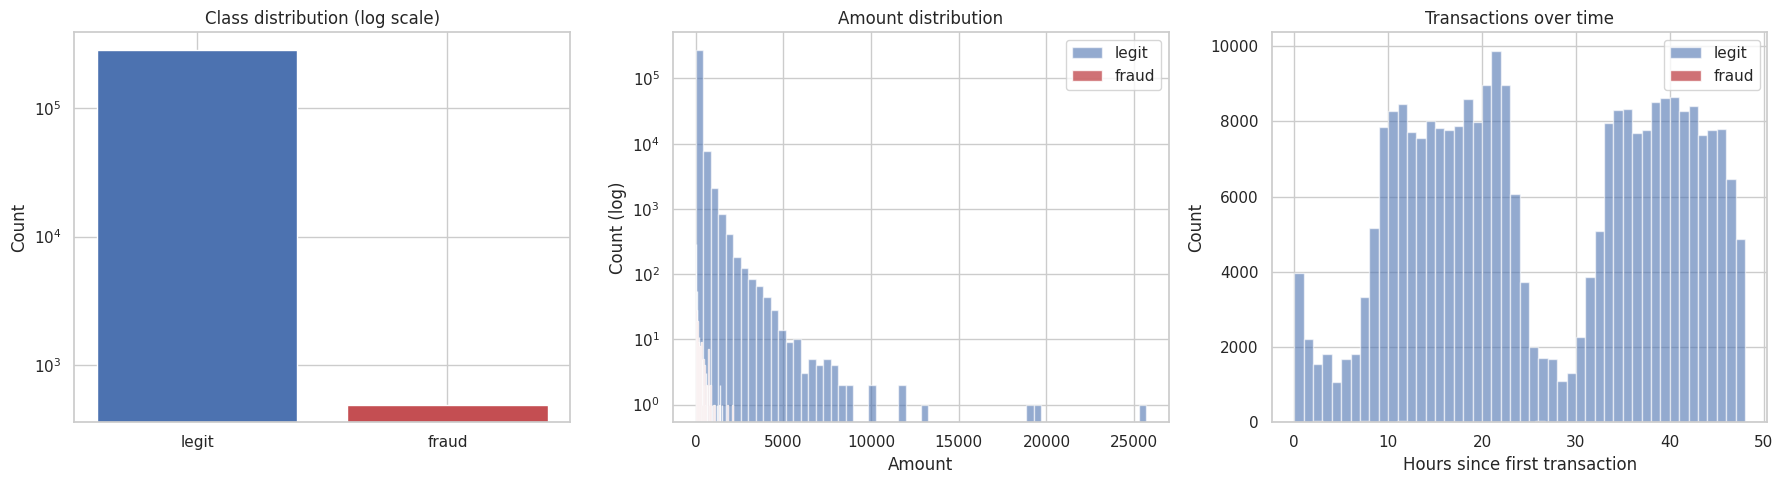
\includegraphics[width=\linewidth]{eda.png}
\caption{Exploratory view of the ULB dataset. Left: class distribution on a log scale (fraud is 0.17\% of total). Middle: \texttt{Amount} distribution for ham and spam on a log y-axis. Fraud amounts are distinct from legitimate amounts but the overlap is substantial. Right: number of transactions per hour over the 48-hour collection window, separated by class. Fraud is clustered but present throughout the window, which motivates both the time-ordered split and the time-window aggregate features.}
\label{fig:eda}
\end{figure}

\section{Methods}

\subsection{Feature sets}

We construct three feature sets on top of the raw columns.

\textbf{The base set} contains the 28 PCA features plus \texttt{Amount}, the features every naive classifier receives. \textbf{The +Benford set} extends base with nine one-hot columns encoding the leading digit (1 through 9) of \texttt{Amount}. \textbf{The full set} extends +Benford with five time-window aggregates: transaction count in the last 60 and 600 seconds, sum of \texttt{Amount} in the last 600 seconds, time since the previous transaction, and a rolling z-score of \texttt{Amount} over 600 seconds.

The time-window features are computed on the entire dataframe before the split. That means the first rows of val and test see history from the end of train. This is not a leakage bug. It mirrors a production system where recent history is always available at inference time, but we flag it here as a deliberate design choice and revisit it in the limitations.

\subsection{Models}

We train seven supervised classifiers and one unsupervised anomaly model.

\begin{enumerate}
\item Logistic regression on base features, unweighted.
\item Logistic regression on base features, \texttt{class\_weight="balanced"}.
\item Logistic regression on +Benford, balanced.
\item Logistic regression on full, balanced.
\item XGBoost on full, untuned, with \texttt{scale\_pos\_weight} set to the training class ratio ($\approx$518).
\item LightGBM on full, untuned, with \texttt{class\_weight="balanced"}.
\item Two-layer MLP with hidden layers $(64, 32)$ on full, wrapped in a \texttt{StandardScaler} pipeline.
\item Autoencoder with latent dimension 8 trained only on legitimate rows, scoring by reconstruction error. Twenty epochs of Adam at learning rate $10^{-3}$, batch size 512.
\end{enumerate}

Models 9 and 10 are tuned variants of LightGBM and XGBoost selected by validation AUPRC from a small grid (see Section~\ref{sec:experiments}). Models 11 and 12 repeat the tuned LightGBM on the base and +Benford feature sets to isolate what each engineered feature family contributes.

\subsection{Evaluation}

We report AUPRC (area under the precision-recall curve), ROC-AUC, and precision at 80\% recall ($P@R{=}0.80$). The last metric is the one that matters for deployment: it answers the question ``if we tune the threshold to catch 80\% of frauds, how many false positives does the team see?'' AUPRC ranks the whole curve and can hide poor behaviour at the operating point. We also report best-F1 threshold and the confusion matrix at that threshold for the winning model.

\section{Experiments}
\label{sec:experiments}

\subsection{Hyperparameter sweep}

For LightGBM we sweep a 16-configuration grid: \texttt{n\_estimators} $\in \{200, 500\}$, \texttt{learning\_rate} $\in \{0.05, 0.1\}$, \texttt{num\_leaves} $\in \{31, 127\}$, \texttt{class\_weight} $\in \{\text{None}, \text{balanced}\}$. The winner on validation AUPRC is $(500, 0.1, 31, \text{balanced})$ at val AUPRC 0.849 and val $P@R{=}0.80$ of 0.931.

For XGBoost we sweep an 18-configuration grid: \texttt{n\_estimators} $\in \{200, 500\}$, \texttt{max\_depth} $\in \{4, 6, 8\}$, \texttt{scale\_pos\_weight} $\in \{1, 10, \text{class ratio}\}$, \texttt{learning\_rate} $= 0.1$. The winner is $(200, 6, 1, 0.1)$ at val AUPRC 0.851 and val $P@R{=}0.80$ of 1.000. The sweep showed that moderate positive-class weights dominate the naive ``match the class ratio'' choice on validation, a known pathology of naive class reweighting in gradient-boosted trees.

Neither grid is exhaustive. They are proof-of-concept sweeps on a fixed $\alpha{=}0.1$ learning-rate family. A production system would use larger grids, Bayesian optimisation, and repeated cross-validation.

\subsection{Training protocol}

All models are trained on the 199{,}364-row train slice and evaluated on the 56{,}962-row test slice. The tuned variants are retrained on train alone after hyperparameter selection, not on train+val combined. This keeps them directly comparable to the untuned baselines on the same training data. The autoencoder is trained only on the legit rows within train, then scored on the full test slice including the 75 held-out fraud cases.

\section{Results}
\label{sec:results}

\begin{table}[h]
\centering
\small
\caption{Test-set results for all models. AUPRC is the primary ranking metric and $P@R{=}0.80$ is the practical operating-point metric. The winning row is in bold.}
\label{tab:results}
\begin{tabular}{lrrrr}
\toprule
Model & AUPRC & ROC-AUC & $P@R{=}0.80$ & Best F1 \\
\midrule
\textbf{7. MLP (full, scaled)}        & \textbf{0.8161} & 0.9757 & \textbf{0.8333} & \textbf{0.8529} \\
12. LightGBM (+ Benford, tuned)       & 0.8077 & 0.9803 & 0.6250 & 0.8296 \\
6. LightGBM (full, untuned)           & 0.8014 & 0.9821 & 0.5405 & 0.8235 \\
9. LightGBM (full, tuned)             & 0.7959 & 0.9792 & 0.5505 & 0.8421 \\
11. LightGBM (base only, tuned)       & 0.7834 & 0.9742 & 0.3659 & 0.8148 \\
5. XGBoost (full, untuned)            & 0.7774 & 0.9780 & 0.2135 & 0.7815 \\
3. LR (+ Benford, balanced)           & 0.7484 & 0.9814 & 0.4511 & 0.7368 \\
2. LR (base, balanced)                & 0.7461 & 0.9831 & 0.4688 & 0.7368 \\
1. LR (base)                          & 0.7119 & 0.9747 & 0.5128 & 0.7429 \\
4. LR (full, balanced)                & 0.7084 & 0.9833 & 0.5310 & 0.7000 \\
10. XGBoost (full, tuned)             & 0.6789 & 0.9648 & 0.1527 & 0.6667 \\
8. Autoencoder (full)                 & 0.1155 & 0.9180 & 0.0648 & 0.2388 \\
\bottomrule
\end{tabular}
\end{table}

\subsection{Headline}

The scaled MLP is the best model on every metric we care about. It catches 58 of the 75 fraud cases in the test slice while flagging only 3 legitimate transactions, for a best-F1 of 0.853 at threshold 0.416. The confusion matrix at that threshold is $\begin{bmatrix} 56884 & 3 \\ 17 & 58 \end{bmatrix}$ (rows are the true label, columns are the predicted label, order is legit then fraud). Figures~\ref{fig:pr} and~\ref{fig:roc} show the precision-recall and ROC curves for every model.

\begin{figure}[h]
\centering
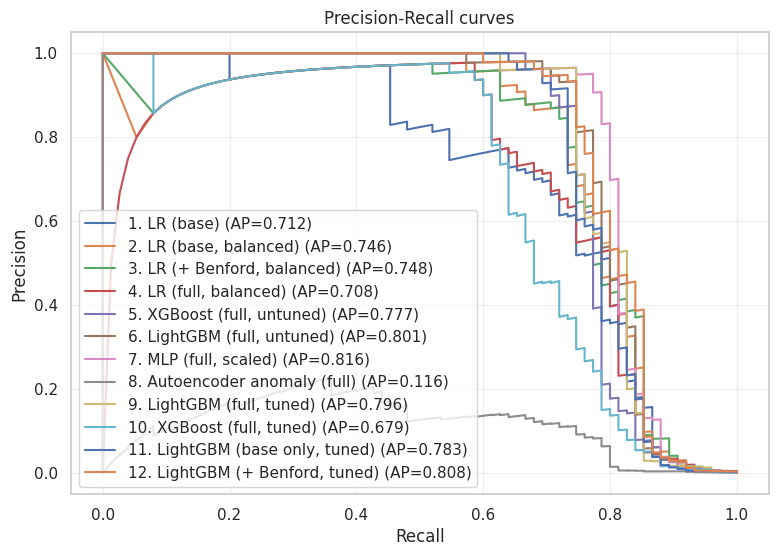
\includegraphics[width=0.9\linewidth]{pr_curves.png}
\caption{Precision-recall curves for all twelve models on the held-out test slice. The MLP and the tuned LightGBM variants dominate the upper right. The autoencoder is the bottom curve, collapsing below 0.2 precision across most of the recall range. The untuned XGBoost and tuned XGBoost curves show the calibration collapse visible in Table~\ref{tab:results}.}
\label{fig:pr}
\end{figure}

\begin{figure}[h]
\centering
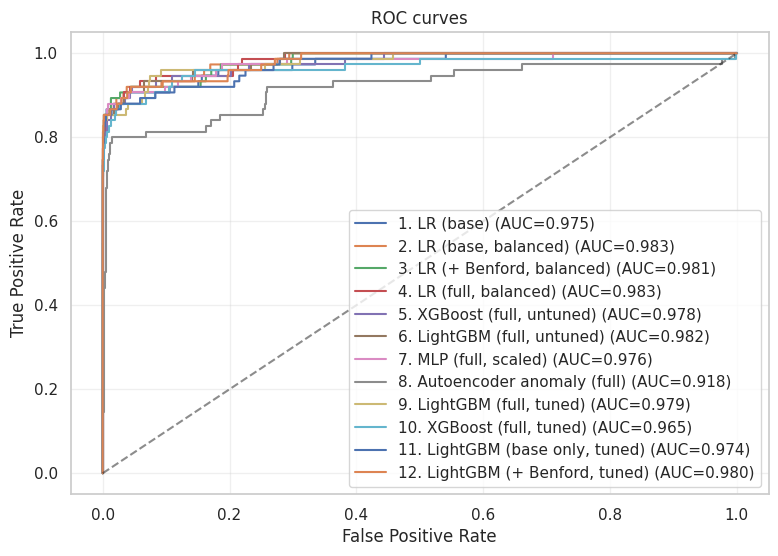
\includegraphics[width=0.9\linewidth]{roc_curves.png}
\caption{ROC curves for all twelve models on the held-out test slice. Note that the ROC curves look much more similar than the precision-recall curves: ROC-AUC is near 0.98 for every supervised model and it hides the differences that matter at the operating point. This is a standard warning about the limitations of ROC-AUC on imbalanced datasets.}
\label{fig:roc}
\end{figure}

\subsection{Benford's Law as a diagnostic}

Before training any model we measured the chi-square distance between the empirical leading-digit distribution of \texttt{Amount} and the Benford prediction $P(d) = \log_{10}(1 + 1/d)$ for each class:
\begin{center}
\begin{tabular}{lr}
\toprule
Subset & $\chi^2$ distance from Benford \\
\midrule
All transactions & 0.0397 \\
Legitimate only  & 0.0395 \\
Fraud only       & 0.2743 \\
\bottomrule
\end{tabular}
\end{center}
Fraud amounts are 6.9$\times$ more distant from Benford's predicted distribution than legitimate amounts. That is a univariate, classifier-free fingerprint of fraud on this dataset. It does not directly win a classification competition, but it validates that a leading-digit feature carries real signal. Figure~\ref{fig:benford} shows the three empirical distributions with the Benford prediction overlaid.

\begin{figure}[h]
\centering
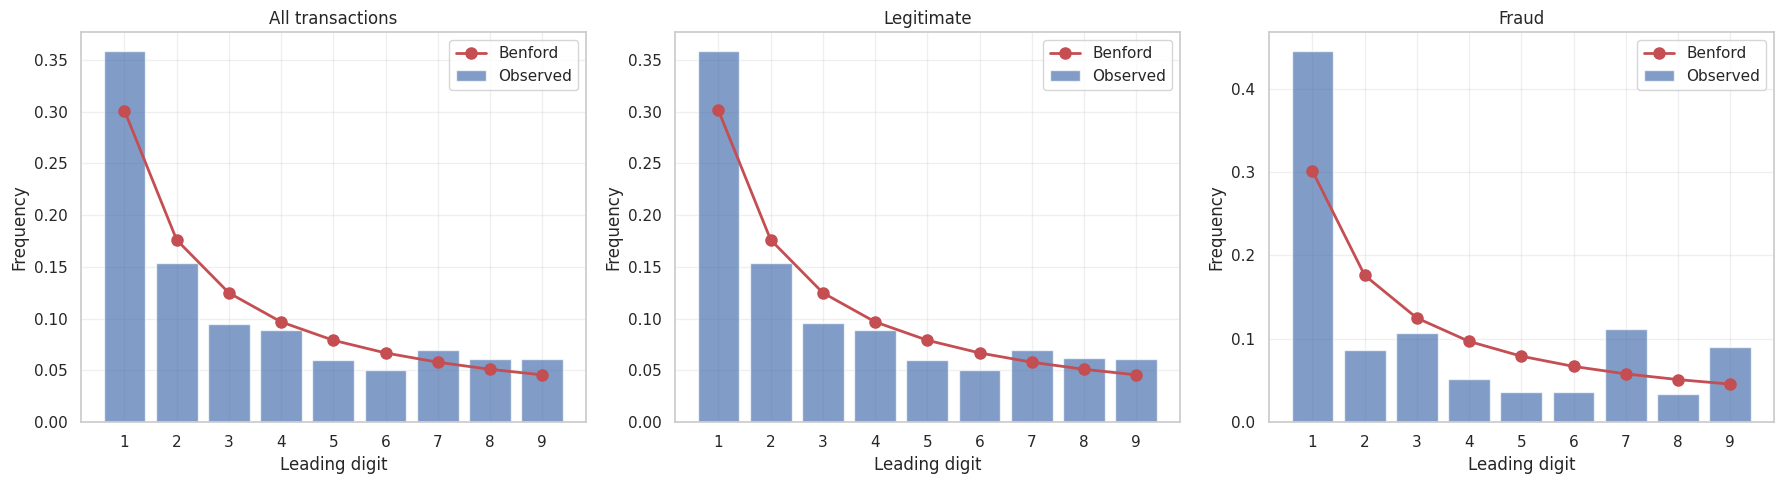
\includegraphics[width=\linewidth]{benford.png}
\caption{Leading-digit distribution of \texttt{Amount}. Left panel: all transactions. Middle panel: legitimate only. Right panel: fraud only. The red curve in each panel is Benford's predicted distribution. The legitimate and overall distributions track Benford closely. The fraud distribution visibly departs from it, which produces the 6.9$\times$ chi-square gap reported in the text.}
\label{fig:benford}
\end{figure}

\subsection{What helps logistic regression}

Starting from the unweighted baseline (AUPRC 0.7119), adding \texttt{class\_weight="balanced"} gives the single biggest lift on this model family and pushes AUPRC to 0.7461. Layering Benford features on top adds another 0.0023 (to 0.7484). Adding the time-window features on top of that drops AUPRC back down to 0.7084, worse than the balanced LR without them. The time-window features are net-negative for LR on this dataset.

\subsection{What helps gradient-boosted trees}

The ablation is cleaner:
\begin{center}
\begin{tabular}{lrr}
\toprule
Feature set (tuned LightGBM) & AUPRC & $P@R{=}0.80$ \\
\midrule
base (PCA + Amount)     & 0.7834 & 0.3659 \\
+ Benford               & \textbf{0.8077} & \textbf{0.6250} \\
+ Benford + time window & 0.7959 & 0.5505 \\
\bottomrule
\end{tabular}
\end{center}
Adding Benford features to a tuned LightGBM lifts AUPRC by 0.024 and precision at 80\% recall by 0.26. Adding time-window features on top of Benford removes about a third of that gain. The story is consistent across LR and LightGBM: the Benford features are a small but genuine win. The time-window features are noise on this dataset.

\subsection{The XGBoost validation-test gap}

XGBoost is the cautionary tale. The untuned model reaches test AUPRC 0.7774. The sweep's winner on validation (AUPRC 0.851, $P@R{=}0.80$ of 1.00) drops to test AUPRC 0.6789 and $P@R{=}0.80$ of 0.153 when retrained on train and evaluated on test. The tuned model is worse than the untuned one on the test slice.

We attribute this to a distribution shift between the validation and test slices. The time-ordered split means the val set is hours 34 through 38 of the 48-hour window and the test set is hours 38 through 48. Those contain different fraud attacks, different amount distributions, and different card-testing burst patterns. A configuration that happens to excel on val by memorising its particular fraud signature does not generalise to test. XGBoost with a small number of shallow trees (\texttt{max\_depth=6}, \texttt{n\_estimators=200}) is apparently more susceptible to this than LightGBM with deeper configurations. The lesson: hyperparameter selection on a time-ordered val slice is not a guarantee of test-set improvement, and single-split tuning can actively hurt on drifting data.

\subsection{The autoencoder}

The autoencoder is the genuine outlier. At test AUPRC 0.1155 it is about 7$\times$ worse than any supervised model. Reconstruction error is not the same signal as labelled fraud, and on this dataset it is far too noisy to substitute. We keep it in the table as a lower bound and a reminder that supervised signal is indispensable when labels exist, even when they are rare.

\section{Discussion}
\label{sec:discussion}

\subsection{What we learned that contradicted our prior beliefs}

Three results surprised us.

\textbf{The MLP beat the tuned gradient-boosted trees on this dataset.} We started with the working assumption that tree models are the hardest baseline to beat on tabular fraud data of this size. The scaled MLP edged LightGBM out on every metric. We do not think this generalises beyond this dataset and it certainly does not on the larger IEEE-CIS dataset where trees typically win by clear margins. On ULB at this particular split the neural model was best.

\textbf{Time-window features hurt.} We expected the Stripe-inspired rolling-window aggregates to be the largest single gain. They were net-negative on LR and they removed part of the Benford lift on the best LightGBM variant. We attribute this to the absence of card or user identifiers in the ULB dataset: our rolling windows aggregate globally across all cards, so a burst in the 60-second window is dominated by high-volume merchants rather than by one card being tested. Stripe's gains come from per-entity sequences, which the public ULB dataset cannot support. The experiment still has value because it falsifies a common reasoning-by-analogy move: ``if sequence features help at Stripe they should help here''. On this dataset they do not.

\textbf{Hyperparameter tuning made XGBoost worse.} This is the XGBoost validation-test gap from Section~\ref{sec:results}. The validation winner lost 0.10 AUPRC and 0.85 on precision at 80\% recall when evaluated on the held-out test slice. Single-split tuning on a time-ordered val set is risky when the data has drift at the timescale of the split. A production system would use rolling evaluation windows; this project had neither the scope nor the data to do that properly.

\subsection{Stripe, honestly}

Our time-window features are a weak approximation of what Stripe describes in their engineering post \cite{stripeflywheel2024}. The Stripe Payments Foundation Model is a large transformer trained on sequences of transaction embeddings at Stripe-scale data volumes. We have no per-card grouping, no self-supervised pretraining, and no sequence model at all. What we have is a handful of rolling-window aggregate features computed globally. The fact that they hurt on this dataset does not disprove Stripe's approach. It shows that the structural requirements of their approach (per-entity sequences, learned representations, large-scale pretraining) are load-bearing. You cannot reproduce the magnitude of their gains on a public dataset that lacks those ingredients.

\subsection{Biases in the evaluation}

Three biases affect how we should read Table~\ref{tab:results}.

\textbf{Test-slice idiosyncrasy.} With only 75 fraud rows in the test slice, AUPRC differences of 0.01 are within the noise of which specific frauds land in the test window. A different time-ordered split would produce different numbers, and we did not average across multiple splits.

\textbf{Benford works on \texttt{Amount}, not on arbitrary tabular features.} Benford's Law applies to quantities that span orders of magnitude. Our features apply it to \texttt{Amount}, which does span orders of magnitude on this dataset. Results will not transfer to domains where the dominant numerical feature is bounded or uniformly distributed.

\textbf{Threshold selection for the confusion matrix.} We report the best-F1 threshold for the winning model. Other threshold choices (maximum Youden, fixed false-positive rate, cost-sensitive) would produce different confusion matrices and different operational implications.

\section{Limitations}

\paragraph{PCA-anonymised features.} \texttt{V1} through \texttt{V28} are principal components. Domain-aware feature engineering is impossible. Any improvement over the base features has to come from the two columns we can read (\texttt{Time}, \texttt{Amount}) or from the modelling side.

\paragraph{No card or user identifiers.} The ULB dataset carries none. We cannot compute per-card velocity features, per-card rolling counts, or per-user anomaly scores. This cripples any faithful reproduction of a sequence-aware fraud system and forces our time-window features to aggregate globally.

\paragraph{Single time-ordered split, not rolling evaluation.} Production fraud systems retrain on sliding windows. Our single 70/10/20 split fixes the train, val, and test periods in advance. The XGBoost validation-test gap shows exactly what goes wrong under this protocol when the val and test distributions drift.

\paragraph{Small hyperparameter grids.} 16 LightGBM configurations and 18 XGBoost configurations do not cover the plausible hyperparameter space. A real tuning run would use larger random search or Bayesian optimisation, at least for the neural model, which got no tuning at all in this report.

\paragraph{Single dataset.} Results on ULB do not generalise to modern payments fraud, which differs in vocabulary, attack patterns, and the ratio of card-testing to card-not-present fraud. The dataset is from 2013. The fraud distribution has moved on.

\section{Reproducibility and code structure}

The project is hosted at \url{https://github.com/dutch-casa/fraud-benford}. The repository layout separates importable modules from the Colab-runnable notebook.

\begin{itemize}
\item \texttt{notebook/fraud\_classifier.ipynb} is the deliverable. Running all cells on a fresh Colab runtime clones the repo, installs dependencies from \texttt{requirements.txt}, loads the dataset directly from a public Google Storage URL, and runs every experiment in this report end-to-end.
\item \texttt{src/data.py} loads the ULB dataset and performs the time-ordered three-way split. \texttt{FraudSplit} and \texttt{FraudSplit3} are frozen dataclasses.
\item \texttt{src/benford.py} implements leading-digit extraction, empirical distribution computation, chi-square distance, and one-hot feature construction.
\item \texttt{src/features.py} implements the five time-window aggregate features using pandas time-indexed rolling operations.
\item \texttt{src/models.py} wraps the five supervised model families plus the autoencoder behind a uniform \texttt{fit}/\texttt{predict\_proba} protocol. The autoencoder is a PyTorch module.
\item \texttt{src/evaluation.py} computes AUPRC, ROC-AUC, precision-recall curves, and the Benford histogram diagnostic plot.
\item \texttt{README.md} documents the run-on-Colab workflow and the repository layout.
\end{itemize}

Each module has typed function signatures and Hoare-style contracts encoded as runtime assertions where they are non-trivial. The code is organised to follow an invariant-first and data-oriented style: data structures define the shape of each stage of the pipeline; functions transform one stage into the next; shared state is avoided.

\section{Collaboration and tools}

This is a team submission by Dutch Casadaban, Brandon Buckley, Carson Phillips, and Devon Li. Work on the notebook, modules, experiments, and report was shared across the team.

Tools used in the development of the code and report: Python 3.11, pandas, numpy, scipy, scikit-learn, xgboost, lightgbm, pytorch, matplotlib, seaborn. LaTeX for the report. Git and GitHub for version control. Google Colab for notebook execution. An AI coding assistant (Anthropic's Claude) was used for pair programming, code review, and prose editing throughout the project. All experimental results are reproduced from running the notebook and are not hallucinated. All design and research decisions are the team's.

\section{Conclusion}

A scaled MLP on PCA features plus \texttt{Amount}, Benford leading-digit features, and time-window aggregates is the best model in our comparison at test AUPRC 0.8161 and precision at 80\% recall of 0.833. A tuned LightGBM with Benford features only is a close second at AUPRC 0.808 with a different trade-off profile. Benford features are a small but consistent win across model families. The time-window features are a small but consistent loss, which we interpret as the absence of per-entity sequences on this dataset rather than a flaw in the sequence-based approach in general. The XGBoost validation-test gap is a cautionary example of how naive hyperparameter tuning on a single time-ordered split can actively hurt test performance. The next step for a follow-up project would be to repeat this experiment on the IEEE-CIS dataset, which carries card and transaction identifiers and would let the time-window aggregates aggregate per card rather than globally. We expect that would flip the sign on the time-window contribution.

\bibliographystyle{plain}
\begin{thebibliography}{9}

\bibitem{dalpozzolo2018}
Dal Pozzolo, A., Boracchi, G., Caelen, O., Alippi, C., and Bontempi, G.
Credit card fraud detection: a realistic modeling and a novel learning strategy.
\textit{IEEE Transactions on Neural Networks and Learning Systems}, 2018.

\bibitem{stripeflywheel2024}
Stripe Engineering.
The ML flywheel: how we continually improve our models to reduce card testing.
\url{https://stripe.com/blog/the-ml-flywheel-how-we-continually-improve-our-models-to-reduce-card-testing}, 2024.

\bibitem{benford1938}
Benford, F.
The law of anomalous numbers.
\textit{Proceedings of the American Philosophical Society}, 78(4):551--572, 1938.

\bibitem{nigrini2012}
Nigrini, M.~J.
\textit{Benford's Law: Applications for Forensic Accounting, Auditing, and Fraud Detection}.
Wiley, 2012.

\end{thebibliography}

\end{document}
